

\section{Grundlagen} % (fold)
\label{sec:grundlagen}

	\subsection{Begriffe}
	\label{sub:begriffe}
		\subsubsection{Pattern und Antipattern} % (fold)
		\label{ssub:pattern_und_anti_pattern}
			"`Entwurfsmuster (englisch design patterns) sind bewährte Lösungsschablonen für wiederkehrende Entwurfsprobleme sowohl in der Architektur als auch in der Softwarearchitektur und -entwicklung. Sie stellen damit eine wiederverwendbare Vorlage zur Problemlösung dar, die in einem bestimmten Zusammenhang einsetzbar ist."'\autocite{pattern15}
			\\

			"`Während "`Design Patterns"' in der Software-Entwicklung allgemein übliche und bekannte Ansätze sind, um Probleme zu lösen, sind Anti-Patterns Negativ-Beispiele – die zeigen, wie man es nicht macht - von bereits durchgeführten, gescheiterten Projekten, die dem erkennenden Mitarbeiter zielgerichtete Hinweise darauf geben, wie die Aufgabenstellung besser gelöst werden könnte. Als Synonym ist auch der Begriff Negativmuster im Gebrauch. Es ist tatsächlich möglich, daß das, was gestern noch als allgemein gangbarer Lösungsweg bezeichnet wurde, heute schon ein "`Antipattern"' ist [...]"' \autocite{Stepken06}

		% subsubsection pattern_und_anti_pattern (end)

		\subsubsection{HTTP-Request Komponenten} % (fold)
		\label{ssub:http_request_komponente}
			\begin{figure}[htbp]
				\begin{center}
					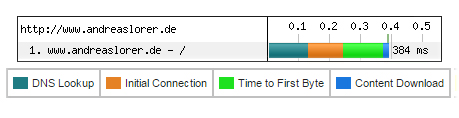
\includegraphics[width=0.6\textwidth]{http_components.jpg}
					\caption{Anfrage der HTML-Datei vom server http://andreaslorer.de (Abbildung nach \url{http://webpagetest.org})}
					\label{fig:http_components}
				\end{center}
			\end{figure}

			\begin{itemize}
				\item DNS Lookup: Um eine Verbindung mit dem Server herzustellen benötigt das HTTP Protokoll die IP Adresse des Ziels. Das heißt beim DNS Server wird für den Namen "`http://andreaslorer.de"' die zu diesem Namen zugehörige IP Adresse zurückgegeben.

				\item Initial Connection bezeichnet die Zeit die vergeht, bis eine Verbindung zum Server hergestellt wurde und eine Kommunikation zwischen Browser und Server stattfinden kann. Hierbei findet der sogenannte TCP "`Three-Way-Handshake"' statt.\footnote{TCP ist das meistgenutzte Verbindungsprotokoll im Internet. Für ein tieferes Verständnis empfiehlt sich dieser Artikel: \href{http://chimera.labs.oreilly.com/books/1230000000545/ch02.html}{High Performance Browser Networking - Chapter 2: Building Blocks of TCP}}

				\begin{figure}[htbp]
					\begin{center}
						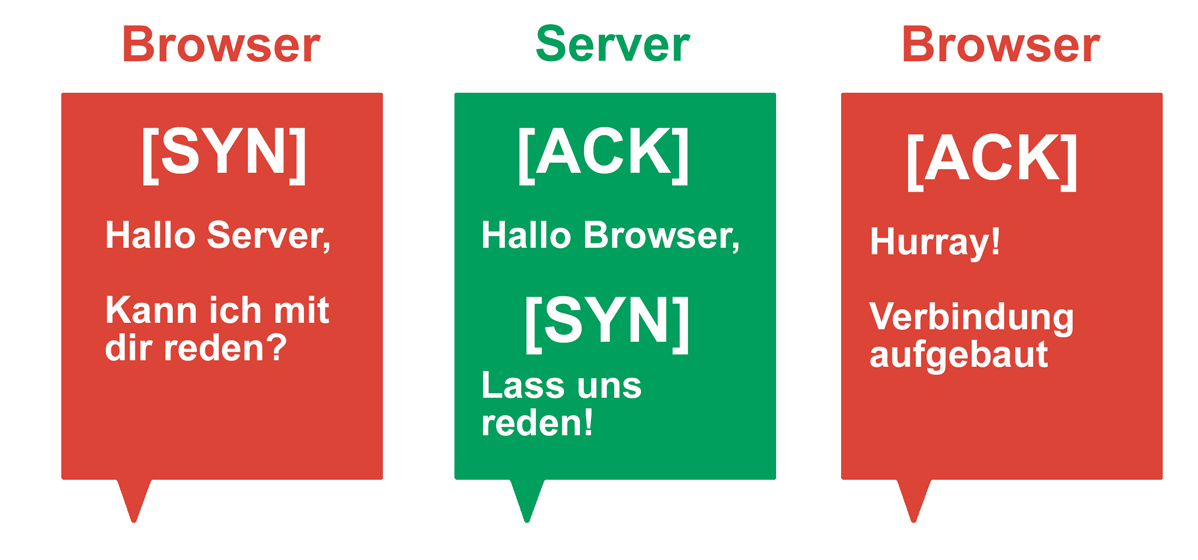
\includegraphics[width=0.6\textwidth]{three_way_handshake.jpg}
						\caption{Three-Way-Handshake zum Aufbau einer TCP Verbindung zwischen Browser und Server (Eigene Abbildung nach: \autocite{bos})}
						\label{fig:three_way_handshake}
					\end{center}
				\end{figure}

				\item TTFB: Ist die Abkürzung für "`Time to first byte"'. Dieser Begriff beschreibt die Zeit die vergeht, bis das erste Byte vom Server beim Browser ankommt. Die Geschwindigkeit und Güte des Servers, Zugriffzeiten auf eine Datenbank oder die Entfernung des Servers können diesen Wert hauptsächlich beeinflussen.

				\item Content Download: Die Zeit die benötigt wird bis die Datei vom Server Heruntergeladen wurde.
			\end{itemize}

			Wie in Abbildung \ref{fig:http_components} zu sehen ist, ist die Zeit für das Herunterladen des HTML Dokuments verschwindend gering im Vergleich zu der Zeit die damit verbracht wurde, um das Herunterladen zu ermöglichen. Dieses Problem ist vor allem auf Smartphones ausschlaggebend dafür, dass Webanwendungen sehr viel langsamer laden als mit einer Kabelverbindung. Das Thema wird in Punkt \ref{sec:netzwerke}: Netzwerke und Latenz noch ausführlicher behandelt.
					
		% subsubsection http_request_komponente (end)

		\subsubsection{Round Trip Time (RTT)} % (fold)
		\label{ssub:rtt}
			"`Round Trip Time"' wird im Deutschen Paketumlaufzeit genannt. Es bezeichnet die Zeit die ein Datenpaket braucht um in einem Netzwerk von Sender A zu Empfänger B und wieder zurück zu gelangen.
		% subsubsection rtt (end)

		\subsubsection{TCP Slow Start} % (fold)
		\label{ssub:tcp_slow_start}

			Ein Round Trip kann nicht beliebig viele Bytes transportieren sondern ist durch die sogenannte "`Congestion Window Size"'\footnote{engl. congestion: Stauung, Überlastung, Anhäufung} limitiert. Der Überbegriff für dieses Verhalten nennt sich "`Slow Start"'

			\begin{figure}[htbp]
				\begin{center}
					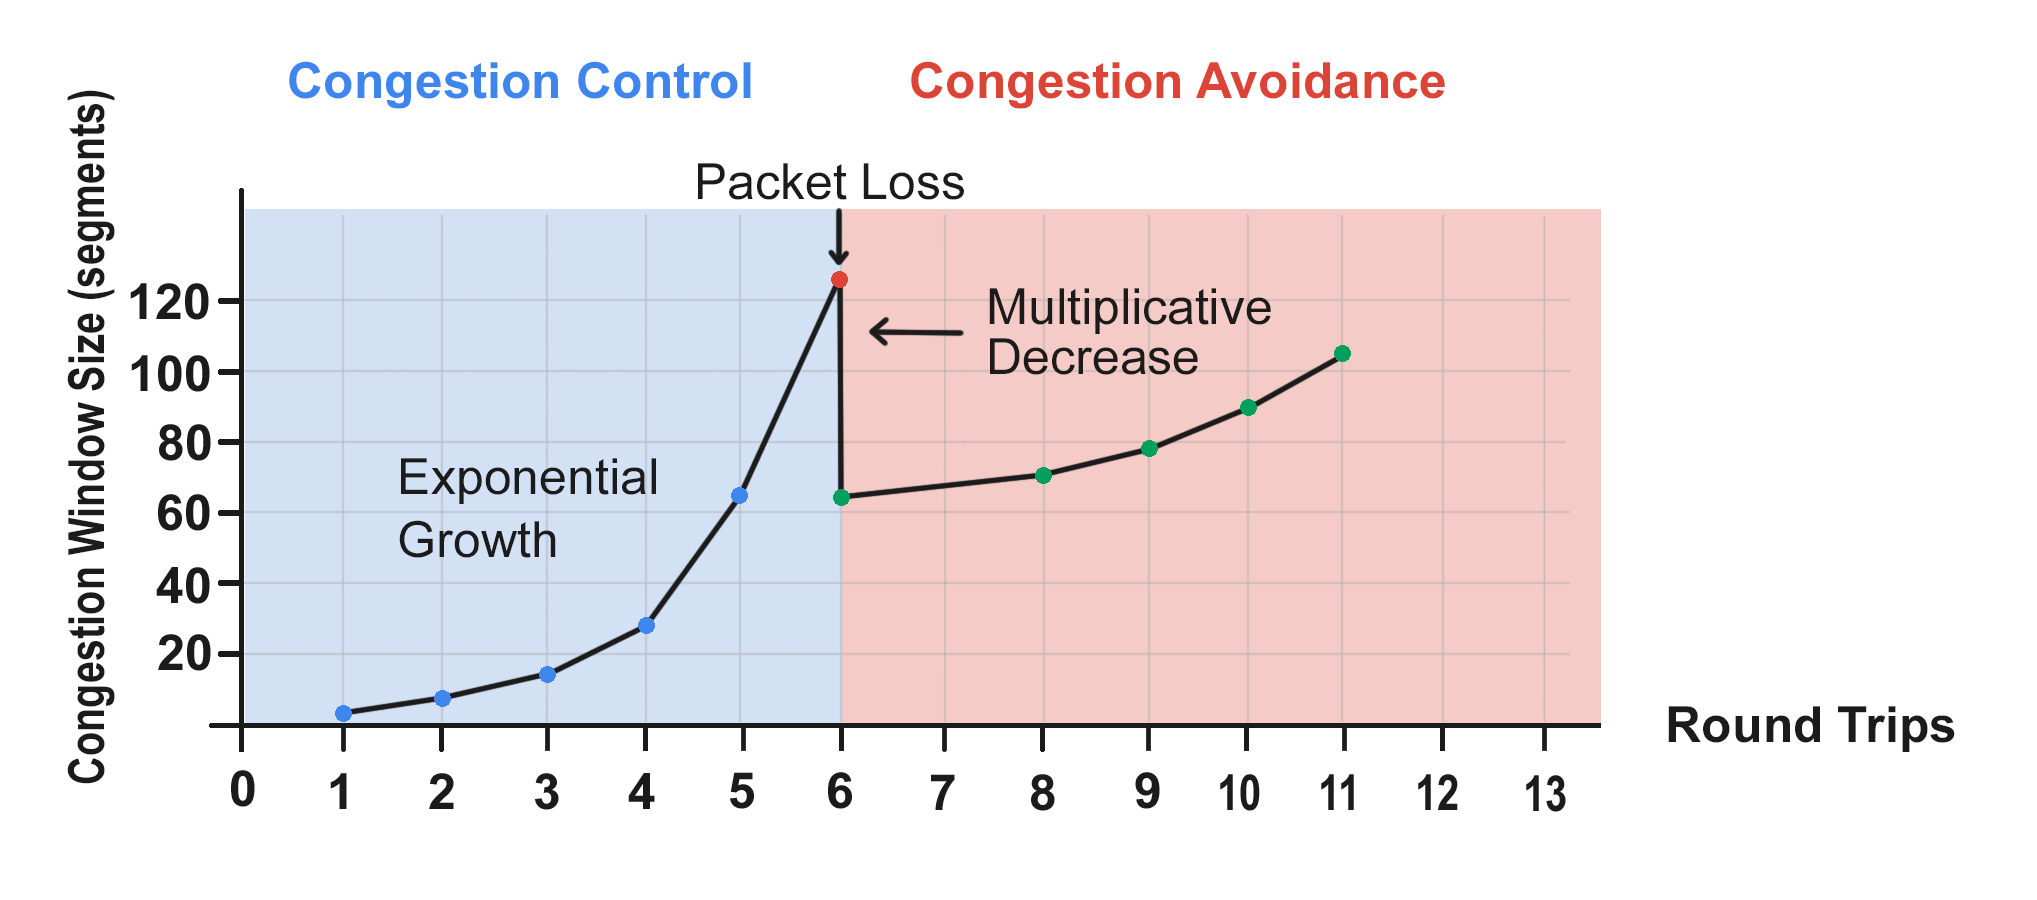
\includegraphics[width=\textwidth]{congestion_window_size.jpg}
					\caption{Congestion Control und Congestion Avoidance (Eigene Abbildung nach \autocite{grigorikSlowStart})}
					\label{fig:congestion_window_size}
				\end{center}
			\end{figure} 

			\begin{itemize}
				\item Congestion Control: Nach dem eine neue Verbindung per TCP aufgebaut wurde, können weder Server noch Client wissen, wie schnell die Verfügbare Bandbreite ist, mit der Daten ausgetauscht werden können. Um das Netzwerk, vor einem Datenstau zu schützen, wird mit einem sehr niedrigen Wert begonnen, der dann ansteigt bis das Limit erreicht ist. Dieses Verhalten nennt sich auch "`Congestion Control"' und verhindert das Aufstauen von Daten.
				\item Congestion Window Size: Diese Größe bestimmt, wieviel Bytes der pro Segmente geschickt werden darf, bis diese vom Empfänger per \texttt{ACK} (acknowledgement) bestätigt werden müssen. Die Größe der Segmente ist Standardmäßig 1460 bytes und die Rate bis zum ACK ist im April 2013 von 4 auf 10 Segmente erhöht worden.\autocite{grigorikSlowStart}. In der Grafik wird davon ausgegangen, das der erste Round Trip 4 Segmente senden darf. Die Datenrate Wächst exponentiell an, damit möglichst schnell die volle Bandbreite nutzbar ist.\\
				\item Congestion Avoidance bedeutet, dass sich die Datenrate wieder um ein Vielfaches verringert, falls es zu einem Paketverlust kommt. Da es besonders bei WLAN oder Mobilfunknetzen des öfteren zu Packetverlusten kommen kann ist dieser Aspekt besonders hervorzuheben, denn er verzögert das erreichen der maximal möglichen Datenrate.
			\end{itemize}

			Slow Start bedeutet also aus sicht der Performance, dass bei einer neuen TCP Verbindung nicht die maximale Bandbreite zu Verfügung steht. Bei größeren Dateien wird zwar durch das exponentielle Wachstum das Maximum schnell erreicht, gerade aber bei kleineren Dateien mit wenigen Kilobyte ist dies oft nicht der Fall.

		% subsubsection tcp_slow_start (end)
		
		\subsubsection{Above The Fold} % (fold)
		\label{ssub:above_the_fold}
			Damit ist der auf einem Bildschirm sichtbare Bereich vor dem Scrollen gemeint. Diesem Bereich wird eine besondere Wichtigkeit zugesprochen.
			\begin{figure}[htbp]
				\begin{center}
					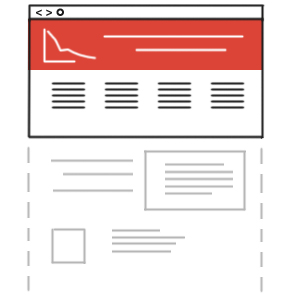
\includegraphics[width=0.3\textwidth]{above_the_fold.jpg}
					\caption{Darstellung des sichtbaren Bereichs vor dem Scrollen}
					\label{fig:above_the_fold}
				\end{center}
			\end{figure}

			\begin{quote}
				 \textit{"`In an analysis of 57,453 eyetracking fixations, we found that there was a dramatic drop-off in user attention at the position of the page fold. Elements above the fold were seen more than elements below the fold: the 100 pixels just above the fold were viewed 102\% more than the 100 pixels just below the fold."'} \autocite{nng15}
			\end{quote}

			Wichtige Informationen oder Navigationselemente sind meistens dort zu finden. Eine Webseite die nach dem Paradigma des Responsive-Webdesign aufgebaut ist kann dabei 3 oder mehrere Ansichten haben die alle einen unterschiedlichen "`above the fold"' bereich haben. Eine Anwendung kann aber auch unterschiedliche Seiten haben, auf dem der Anwender beim Aufrufen der Seite landen kann. Zum Beispiel wenn dieser An- oder Abgemeldet ist. Paradebeispiel dafür sind Facebook oder Twitter.
		% subsubsection above_the_fold (end)

		\subsubsection{Perceived Performance} % (fold)
		\label{sub:perceived_performance}
			\begin{figure}[htbp]
				\begin{center}
					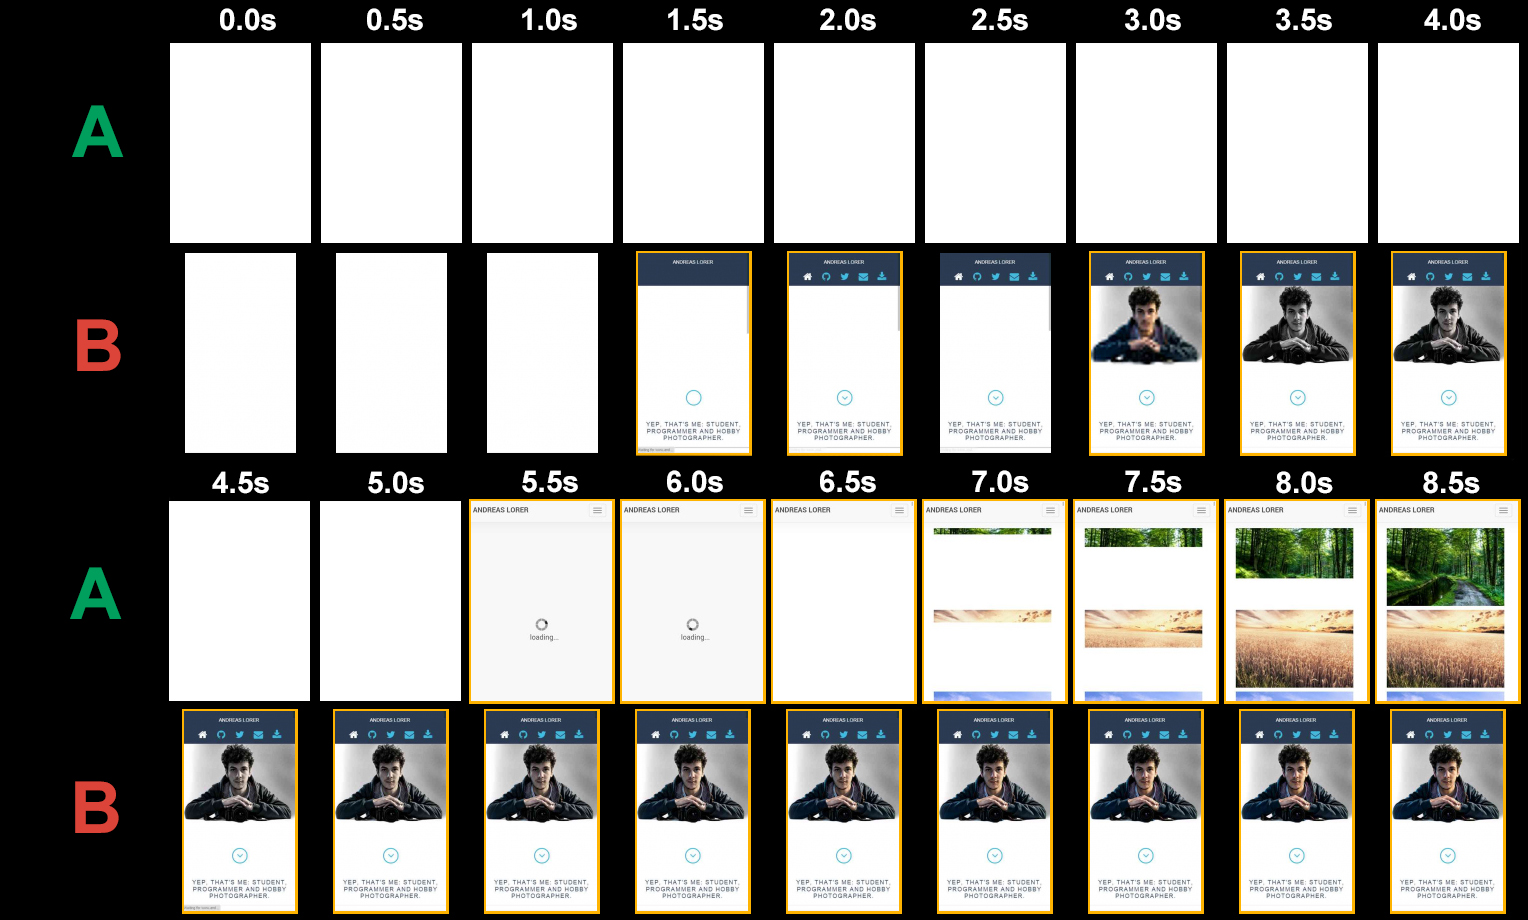
\includegraphics[width=0.9\textwidth]{perceived_performance.jpg}
					\caption{Zwei Seiten im Vergleich (Eigene Abbildung via webpagtest.org)}
					\label{fig:perceived_performance}
				\end{center}
			\end{figure}

			Abbildung \ref{fig:perceived_performance} zeigt die Seiten A und B, mit nahezu identischer Ladezeit. Der Unterschied besteht darin, dass Seite B bereits nach 1.5 Sekunden eine erste visuelles Rückmeldung für den Anwender zu sehen ist wohingegen Seite A erst nach 5.5 Sekunden dem Anwender zeigt, dass sie überhaupt ladet.
			"`Perceived Performance"' steht also für die Zeit bis ein erste visuelle Rückmeldung für den Anwender zu sehen ist und bedeutet, dass die Ladezeit als schneller empfunden wird, als es eigentlich laut Messwerten der Fall ist. Warum diese "`Perceived Performance"' für eine Webanwendung so wichtig ist zeigen mehrere Studien, deren Daten in folgender Infographik aufbereitet sind.

			\begin{figure}[htbp]
				\begin{center}
					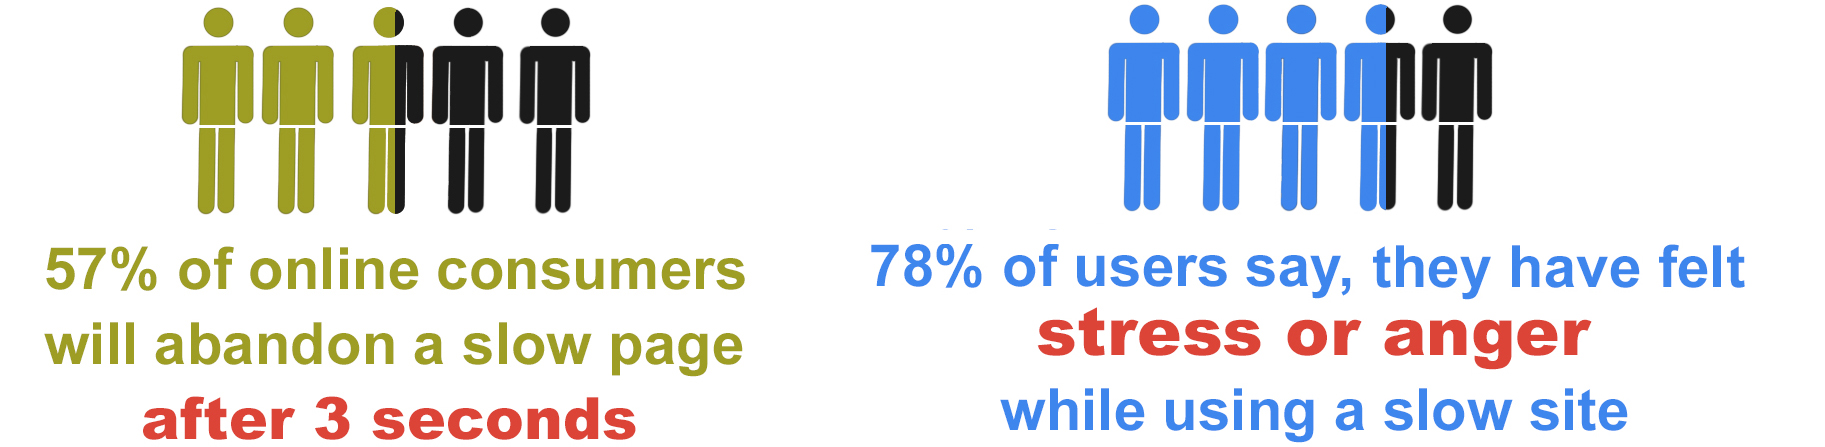
\includegraphics[width=0.7\textwidth]{effect_of_slow_loadtimes.jpg}
					\caption{Einfluss und Effekt einer langsamen Seite auf den Anwender (Eigene Abbildung nach Daten von: \autocite[p. 8]{radware14})}
					\label{fig:effect_of_slow_loadtimes}
				\end{center}
			\end{figure}

			Bereits kleine Verbesser- oder Verschlechterungen der Ladezeit können einen großen Einfluss in auf den Anwender haben. Yahoo hat herausgefunden, dass wenn eine Seite um nur 400 Millisikunden schneller ist, sich der Traffic um 9\% erhöhte.\autocite{stefanov08} 57\% der Online Konsumenten haben eine Seite, die länger als 3 Sekunden ladet bereits wieder verlassen. 78\% der Anwender empfinden sogar Zorn oder Stress wenn eine Seite nicht Ladet oder es nicht ersichtlich ist, dass die Seite reagiert.

		% subsubsection perceived_performance (end)
	% subsection begriffe (end)
\pagebreak
% section grundlagen (end)


\section{Die 1000 ms Barriere} % (fold)
\label{sec:die_1000_ms_barriere}
	Das Ziel dieser Arbeit, die 1000 Millisekunden Barriere zu durchbrechen, wurde nicht durch einen Zufall gewählt. Der Anwender nimmt die Geschwindigkeit einer Seite subjektiv wahr. Sie wird in der folgenden Grafik interpretiert:

	\begin{figure}[htbp]
		\begin{center}
			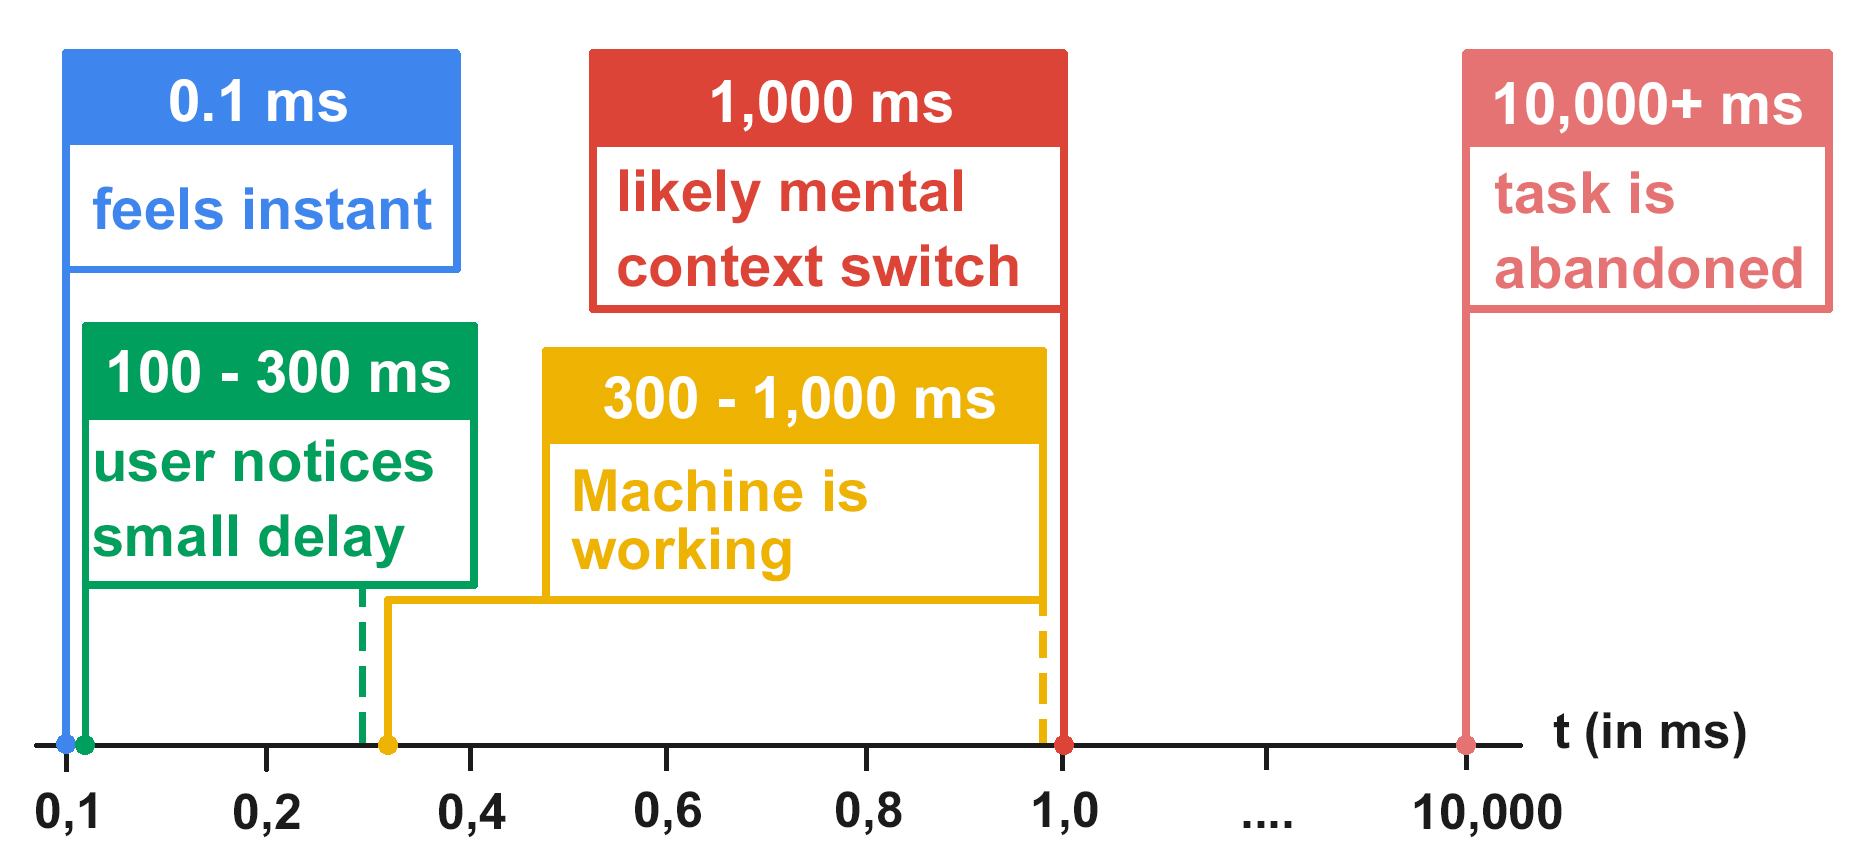
\includegraphics[width=\textwidth]{human_perception.jpg}
			\caption{Zeit und Wahrnehmung durch den Anwender (Abbildung nach Daten von: \autocite{grigorikHumanPerception})}
			\label{fig:human_perception}
		\end{center}
	\end{figure}

	Wie zu sehen ist bleiben gerade einmal eine Sekunde, bevor das Gehirn uns sagt, man solle doch einer anderen Aufgabe nachgehen bis der Ladevorgang abgeschlossen ist. Der Anwender verlangt visuelle Rückmeldung um "`am Ball zu bleiben"', dies wurde bereits in Punkt ~\ref{sub:perceived_performance} "`Perceived Performance"' angesprochen. Auf vielen Webseiten sieht man deshalb, Ladebalken oder sogenannte \texttt{Spinner}, die dem Anwender sagen, dass der Ladevorgang in gange, aber noch nicht abgeschlossen ist.

	Um das Ziel von einer Sekunde Ladezeit bis zum ersten Render zu erreichen, ist es von nöten zu verstehen wo Zeit verloren geht und wie viele Millisekunden am ende noch zur Verfügung stehen um es zu erreichen.\\

	\subsection{Touch Event} % (fold)
	\label{sub:touch_event}
		Der Aufruf einer Seite über das Smartphone erfolgt über ein Touch Event auf einen Link, Button oder die Seite wird per URL aufgerufen. Hierbei können je nach Gerät zwischen 50 (IPhone 5) und 123 Millisekunden (Moto X - Android) an Zeit verloren gehen, bis das Event registriert wurde.\autocite{venturebeat} Der Browser wartet allerdings nochmals bis zu 300 Millisekunden, denn er muss abwarten ob vielleicht noch ein zweiter Finger aufgelegt wird, oder ob der Anwender Scrollen oder Zoomen möchte.\autocite{google11}

		Dieses Verhalten lässt sich bei vielen Browsern per \texttt{Meta Tag} abstellen:

		\begin{lstlisting}
			<meta name="viewport" content="user-scalable=no">
		\end{lstlisting}

		Dies setzt natürlich voraus, dass die Webanwendung kein Zoomen benötigt um sie zu bedienen! Gerade bei älteren Webseiten trifft das oftmals nicht zu. Eine vollständige Liste mit Meta Tags für die verschiedenen Browser ist der Fußnote zu entnehmen.\footnote{Suppressing 300ms delay for touchscreen interactions: \url{http://tinyurl.com/psj5nxz}}

	% subsection touch_event (end)

	\subsection{Netzwerke} % (fold)
	\label{sub:netzwerke}


	\begin{figure}[htbp]
		\begin{center}
			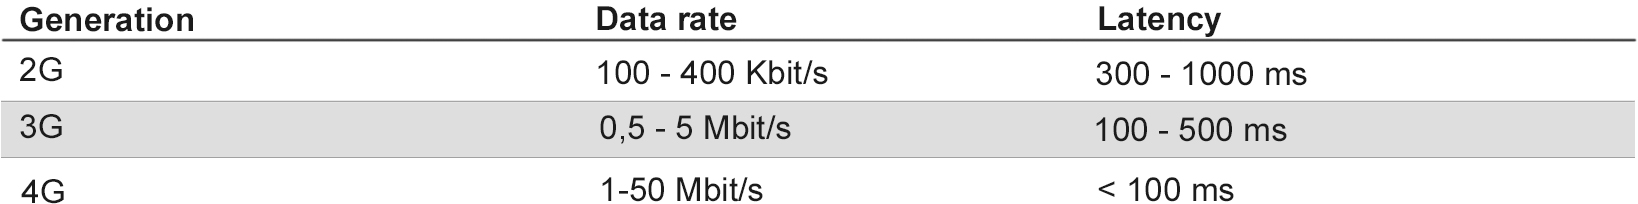
\includegraphics[width=\textwidth]{mobile_networks.jpg}
			\caption{Datenrate und Latenz für eine aktive mobile Verbindung (Eigene Abbildung nach Tabelle \autocite{grigorikGNetwork})}
			\label{fig:mobile_networks}
		\end{center}
	\end{figure}

	% section netzwerke (end)

	% subsection mobile_netzwerke (end)

	\subsubsection{Kritischer Rendering-Pfad} % (fold)
	\label{ssub:critical_render_path}
		Auf Englisch "`critical render path"' genannt, ist der wohl wichtigste Begriff, wenn es um schnelle Ladezeiten geht. Durch die Optimierung des Rendering Pfads kann die benötigte Zeit für das erste Rendern der Seite erheblich verkürzt werden. Das Verständnis des Rendering-Pfads ist zudem eine wesentliche Voraussetzung für die Erstellung von schnellen Webanwendungen und soll in diesem Abschnitt ausführlich erklärt werden. Dabei wird der Begriff in seine zwei Teile Zerlegt: Kritischer und Rendering-Pfad.\\

		Der Rendering-Pfad setzt sich aus den für die Anwendung nötige Ressourcen zusammen. Webanwendungen bestehen meist aus mehreren ausgelagerten Javascript und CSS Dateien die benötigt werden um überhaupt mit dem Rendern zu beginnen. Ein Seitenaufruf erzeugt folgenden Prozess:
		\begin{figure}[htbp]
			\begin{center}
				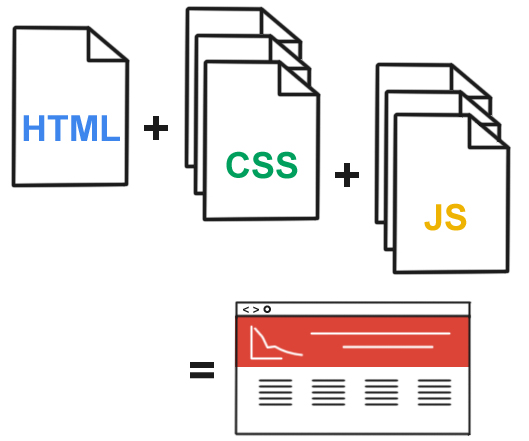
\includegraphics[width=0.4\textwidth]{critical_render_path.jpg}
				\caption{Ressourcen die für das Rendern von nöten sind}
				\label{fig:critical_render_path}
			\end{center}
		\end{figure}

		\begin{enumerate}
			\item Nachdem die Adresse per DNS-Lookup (siehe Punkt: \ref{ssub:http_request_komponente}) in eine IP Adresse übersetzt wurde, wird eine TCP Verbindung hergestellt und der Browser beginnt damit die HTML Datei vom Server zu laden.
			\item Der Browser liest das HTML von oben nach unten und sieht nach, ob zusätzliche Ressourcen benötigt werden (Bilder, Javascript oder CSS).
			\item Diese Ressourcen werden beim Server angefragt.
			\item Der Browser kann mit dem Rendern der Seite noch nicht beginnen, da er noch auf den Abschluss des Downloads wartet.
			\item Der Browser liest das Javascript und sieht nach, welche CSS Selektoren auf das HTML Dokument passen.
			\item Der Browser stellt fest, dass die Seite nun Angezeigt werden kann und beginnt mit dem Rendern.
		\end{enumerate}

		\begin{figure}[htbp]
			\begin{center}
				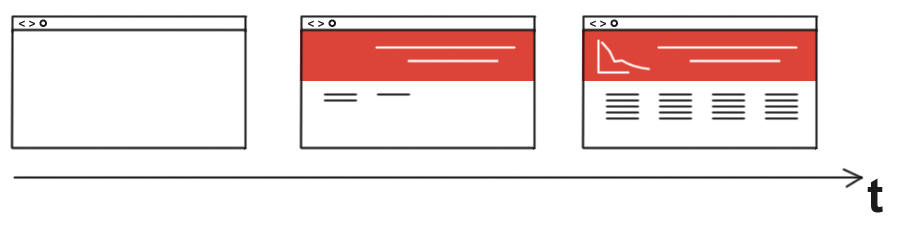
\includegraphics[width=0.75\textwidth]{browser_render.jpg}
				\caption{Der Render Prozess der im Browser abläuft (Eigene Abbildung)}
				\label{fig:browser_render}
			\end{center}
		\end{figure}
	
		Wie im Prozessablauf abgebildet, ist ein frühes Rendering oft nicht möglich, weil Javascript und CSS das Rendern dadurch Blockieren, da sie zuerst Herunterladen werden und dann Übersetzt werden müssen, bevor der Browser entscheiden kann, dass die Seite gerendert werden kann. Kritischer Rendering-Pfad bedeutet, dass dem Browser die Daten zuerst zur Verfügung gestellt werden, die nötig sind um den "`above the fold"' Inhalt zu rendern. Alle anderen Ressourcen sollten erst nach dem Laden der Seite Heruntergeladen werden um das Rendern nicht zu verzögern. 

	% subsubsection critical_render_path (end)


% section die_1000_ms_barriere (end)


\pagebreak
